\chapter[Creation and Training of Spectral ViT]{Creation and Training of the\newline Spectral ViT}
%Ensure that the chapter title fits on the header lines, but doesn't hyphenate on the chapter title page
\label{chap:methods}
% Methods to validate transformers (fake spectra), create training data (fake spectra), 
% train various models (V1.1, V1.2, V1.3, V2), to find optimal training for V2

In order to examine the effectiveness of the transformer architecture for
spectral classification, the following series of steps were taken. First, a custom transformer 
architecture was created based on the traditional ViT architecture \parencite{dosovitskiy2020}, 
and trained on a simple synthetic dataset to validate our approach. Next, a synthetic dataset 
using DESI spectra was created under a variety of preprocessing conditions. The previously 
created CNN and new transformer architectures were trained on the
same preprocessed data. Finally, these training samples were used to determine 
the optimal training conditions for non-redshift corrected data. 

\section{Creation of Spectral ViT}\label{sec:SpecViT}
The Spectral ViT architecture was coded using the \texttt{PyTorch}
deep learning framework~\parencite{PyTorch2019}. The complete architecture is shown graphically in
Appendix~\ref{fig:SpectralViTDiag}. The Spectral ViT is composed of three main components:
the pre-processor, the encoder, and the classifier. 

The pre-processing component is responsible for taking the 
input spectra extracted from the DESI CCDs and converting them into a series of 
vectors that the transformer can interpret. 
Consider a sample of $N$ spectra, each with $10000$ pixels corresponding to a bin containing a wavelength 
between $3600\AA$ and $9800\AA$. Each group is split into a set number of patches 
(approximately 100 pixels in length). Each patch is then 
linearly mapped via a fully connected network to a vector 4 times smaller than the patch size.
The sample is now a set of size $N\times100\times25$. A classification token of the same dimension as the patches 
is initialized with uniformly distributed random values between 0 and 1, and then concatenated to the beginning of each sample.

\begin{figure}[t]
    \centering
    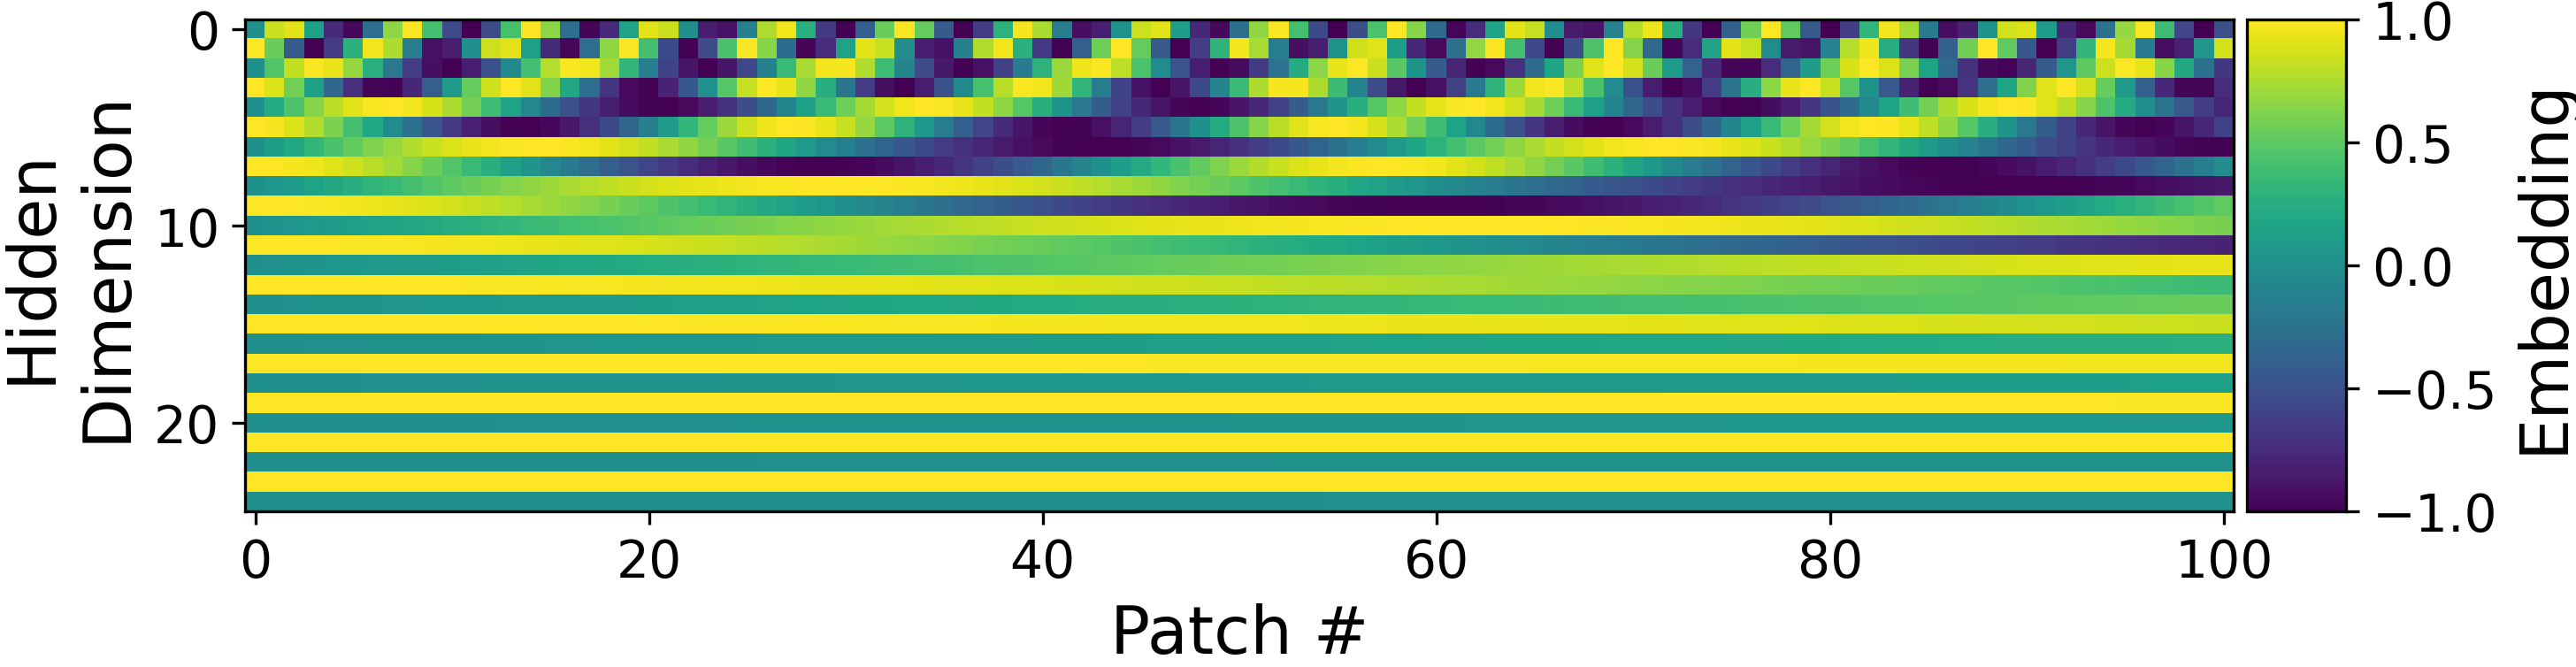
\includegraphics[width=\linewidth]{figures/embeddings_new.png}
    \caption[Positional Embeddings for ViT]{Visual representation of the embeddings for a sample of spectra. The x-axis represents the 
    index of the patch, the y-axis represents the index of the hidden dimension, and the color represents 
the value of the embedding.}
    \label{fig:embedding}
\end{figure}

In order for the transformer to properly understand the positional relationship between each patch, an embedding 
is added to each patch. This embedding is a scalar function based on the size 
of the patch and is calculated as follows: 
\begin{equation}
    \text{Embedding}_{ij} = \begin{cases} \sin\left(\frac{i}{10000^{(j / \text{patch size})}}\right) & \text{if } j \text{ is even} \\
    \cos\left(\frac{i}{10000^{((j - 1) / \text{patch size})}}\right) & \text{if } j \text{ is odd}\end{cases},
\end{equation}
where $i$ is the patch index, $j$ is the index in the hidden dimension, and 
the patch size is the number of pixels defined in each patch \parencite{vaswani2017}. 
In a CNN, the positional relationship between each pixel is understood by the convolutional layers
and the pooling layers. However, in a transformer without the positional embeddings, there is no difference between 
the first and last patch in the sample. The sinusoidal embeddings we use are based on the original transformer architecture \parencite{vaswani2017}, but also provide a simple way to encode the positional information. A visual 
representation of the embeddings for the sample is shown in Fig.~\ref{fig:embedding}. Once the 
embeddings are added element-wise to the patches, the resulting tensor of size $N\times101\times300$ is passed through the encoder. 



The encoder is the main component of any ViT architecture, as it contains the 
multi-head attention and feed-forward layers. The encoder is composed of a user-defined number of
transformer blocks, each of which contains layer normalization, multi-head attention, another 
layer normalization, and finally a feed-forward layer. The multi-head attention layer 
used in this work is a scaled dot-product attention layer found in \textcite{vaswani2017}, with the adjustments suggested by  \textcite{Xiong2020} for efficient training. Each patch 
is passed through three separate linear layers, each with a different set of weights, 
resulting in three sets of vectors: the query ($Q$), key ($K$), and value ($V$).
\begin{equation}
    \label{eq:mhsa}
    \text{Attention}(Q, K, V) = \text{softmax}\left(\frac{Q\cdot K^T}{\sqrt{d_k}}\right)\cdot V
\end{equation}
The dot product between the query and key vectors is then calculated,
scaled by the square root of the dimensionality of the query vector, and then passed through a softmax function,
\begin{equation}
    \text{softmax}(x_i) = \frac{e^{x_i}}{\sum_{j=1}^N e^{x_j}}.
\end{equation}
The resulting attention weights are then multiplied by the value vectors (Equation~\ref{eq:mhsa}). 
This is simultaneously done for each head in the multi-head attention layer. Each result is concatenated together and then passed through a linear layer to reduce the dimensionality
to the size of the query vector. 
\begin{figure}[hb!]
    \centering
    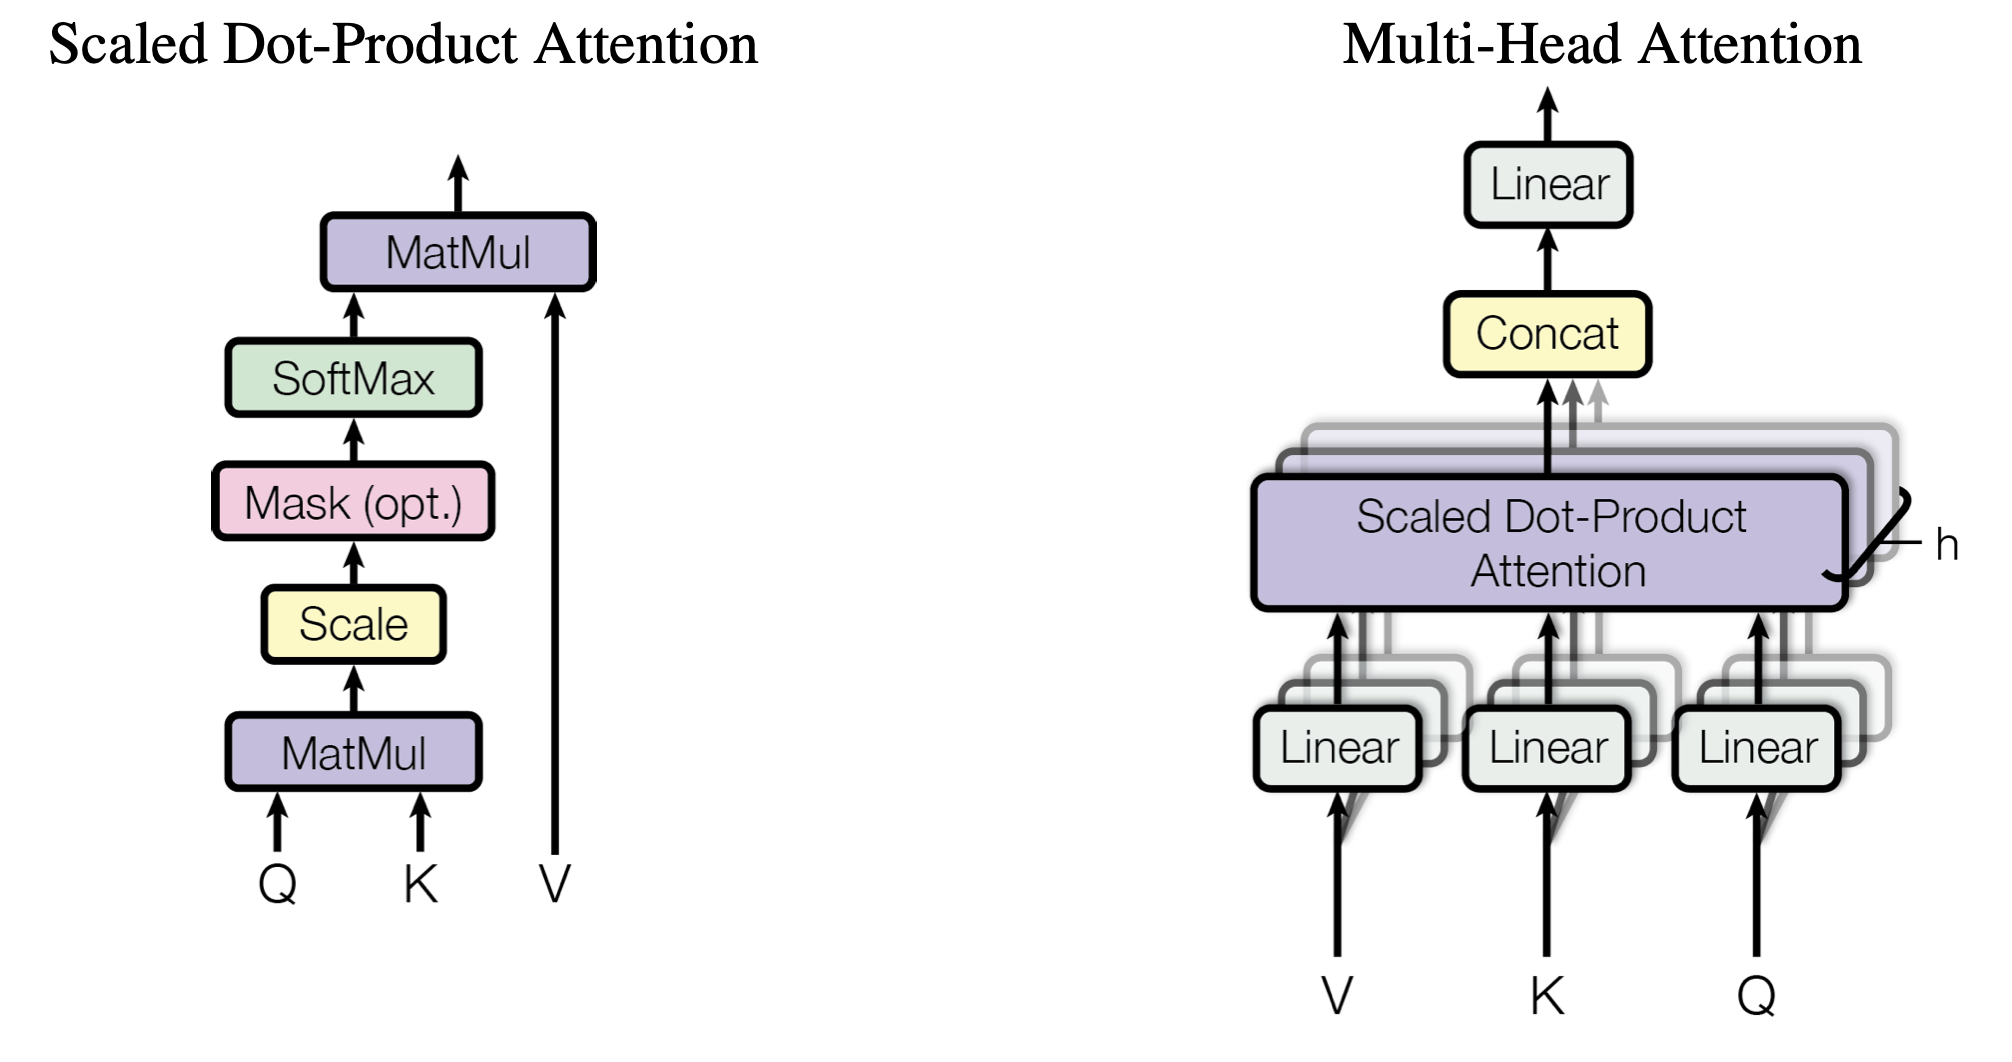
\includegraphics[width=.9\textwidth]{figures/transformer_paper/SelfAttention_MHSA.png}
    \caption[Transformer Attention]{Graphical Depiction of Multi-Head Attention Layers inside a 
    transformer architecture. Image from \textcite{vaswani2017}}
    \label{fig:attention}
\end{figure}
This resulting vector is then added
element-wise to the original patches, normalized, and then passed through a MLP, 
resulting in a tensor of size $N \times 101 \times 300$. This again is added element-wise to the original patches. A 
visual example of this is shown in Figure~\ref{fig:attention}. 
Each step is repeated for a user-defined number of transformer blocks, resulting in a tensor of size
$N \times 101 \times 300$. A diagram of the ViT block used the Spectral ViT is shown in 
Figure~\ref{fig:SpectralViTBlock}. 


The final component of the Spectral ViT architecture is the classifier. The classifier
takes in only the first patch of each sample, which has been designated as the classification token.
The classification token is passed through a linear layer to reduce the dimensionality to the
number of classes, and then passed through a softmax function to produce a probability distribution
over the classes. Therefore, the resulting tensor is of size $N \times 1 \times 6$, for our 
6 classes of galaxy + SNe sub-types.

\subsection{Validation of Spectral ViT Architecture}
\label{ssec:validation}
After creating the Spectral ViT architecture, we tested our  ability to train it 
effectively. A synthetic dataset, consisting of a continuum with 
broad Gaussian peaks placed at predetermined locations, was created. Certain combinations of 
peak locations were chosen to represent an arbitrary `class' of SNe. 
\begin{figure}[t]
    \centering
    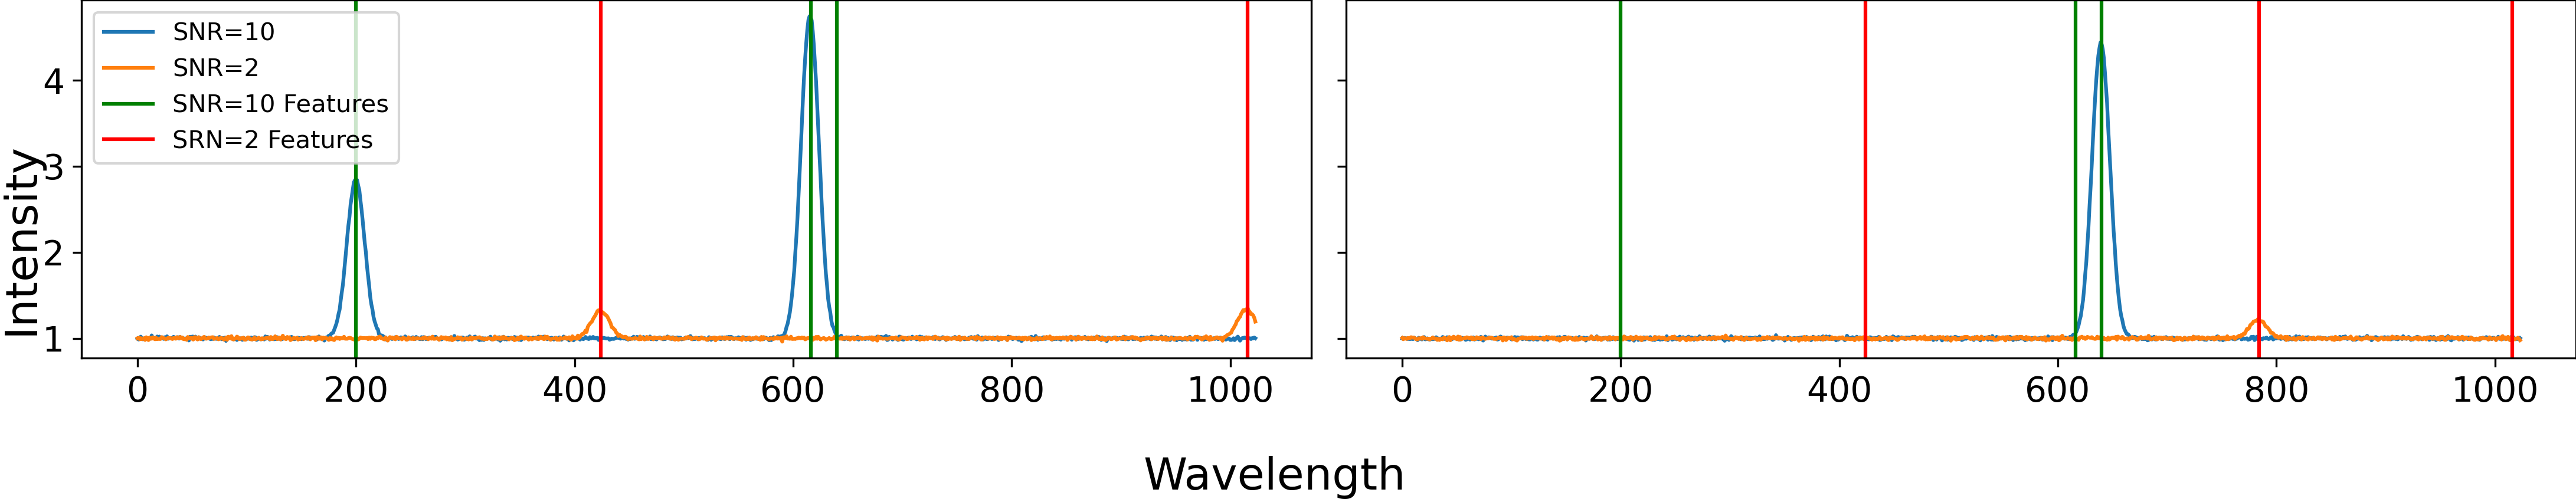
\includegraphics[width=\textwidth]{figures/synth_data_new.png}
    \caption[Synthetic spectra]{Synthetic spectra used to verify the performance of Spectral~ViT. Red and green vertical lines represent features used to 
    separate the data into distinct classes for SNR=2 and SNR=10, respectively. Two classes are shown for each SNR.}
    \label{fig:synth_spectra}
\end{figure}
These peaks, 
our synthetic ``emission lines,'' were given random amplitudes and widths to simulate 
variability based on the maximum `signal' allowed for a given sample. 
To ensure the performance of the model, two sample sets were made: one with particularly noisy data 
(a maximum signal only extending past the Gaussian noise by a factor of 2), and one with 
very prominent features (a maximum signal extending past the Gaussian noise by a factor of 10). For 
convenience, these datasets were labeled to have a signal-to-noise ratio (SNR) of 2 and 10, respectively. 
Examples of the synthetic spectra with different continuum profiles are shown in Fig.~\ref{fig:synth_spectra}. 

These datasets with SNR=10 were trivially separable by a Spectral ViT architecture 
with two transformer blocks, two transformer heads, eight hidden layers, and a patch size of 16 (spectra were 1024 pixels long). 
An accuracy of 100\% on the testing set was achieved within 5 epochs of training (Figure~\ref{fig:snr10}). Trained on the same 
architecture, the data with SNR=2 was more difficult to separate, only achieving a 33.975\% test accuracy (Figure~\ref{fig:snr2}).



% Make into subcaptions
\begin{figure}[t]
    \centering
    \subfloat[\centering~SNR = 2\label{fig:snr2}]{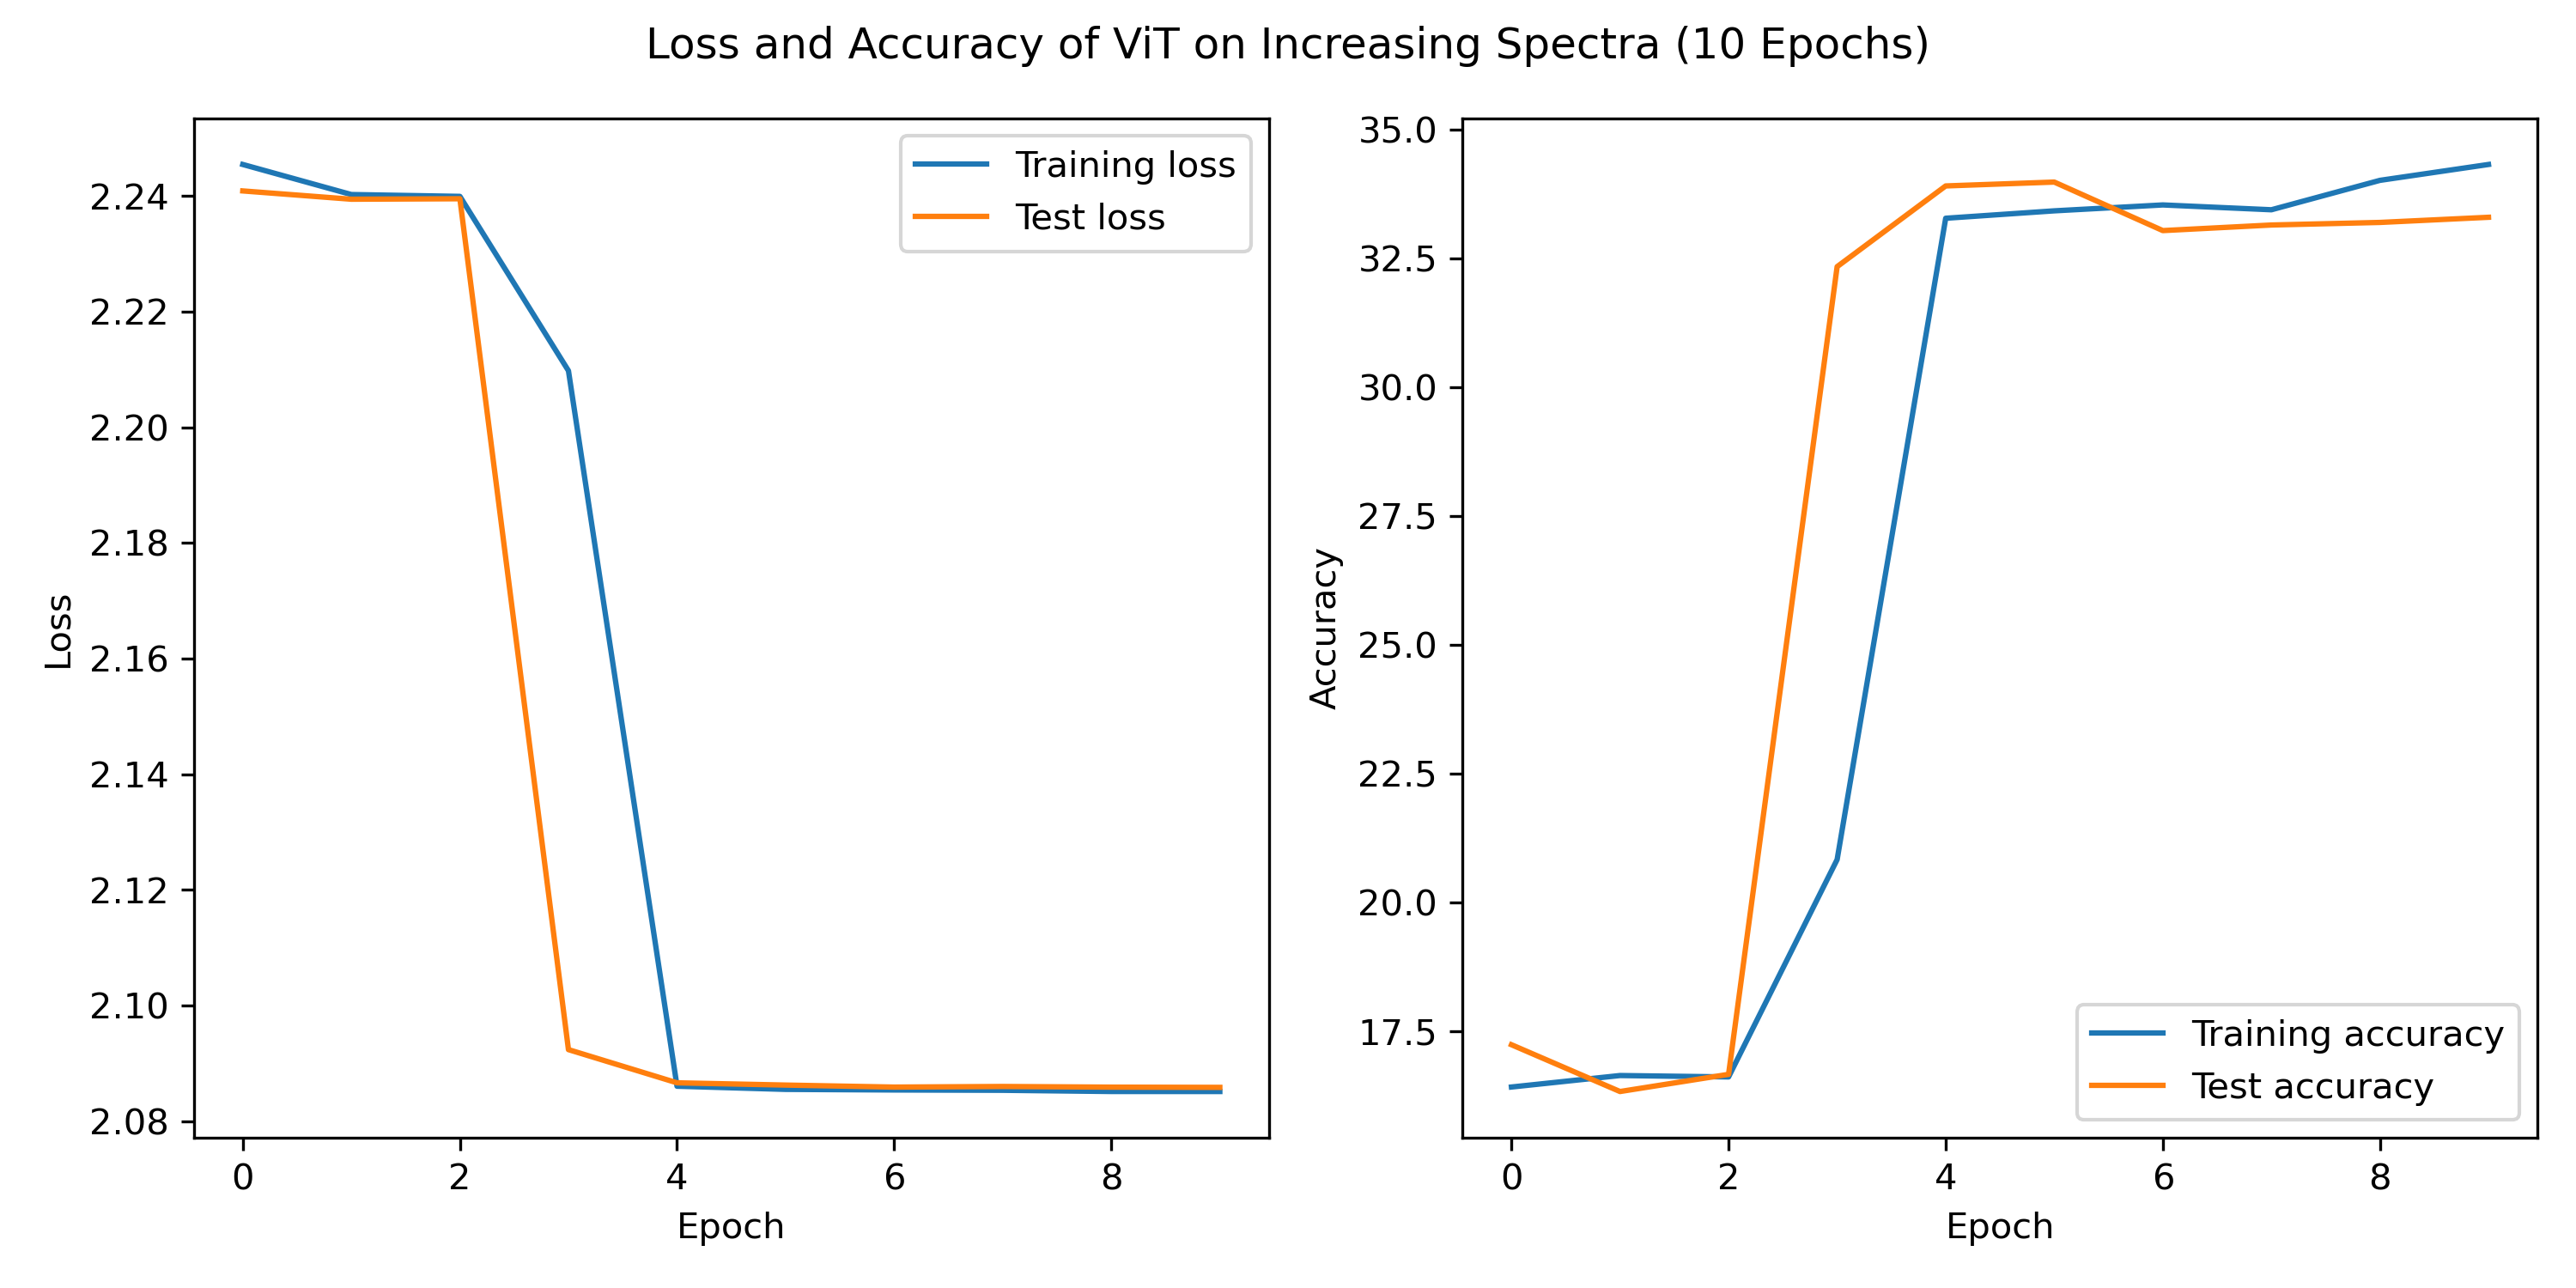
\includegraphics[width=11cm]{figures/pre_testing/SNR2_training_epoch.png}}
    \qquad
    \subfloat[\centering~SNR = 10\label{fig:snr10}]{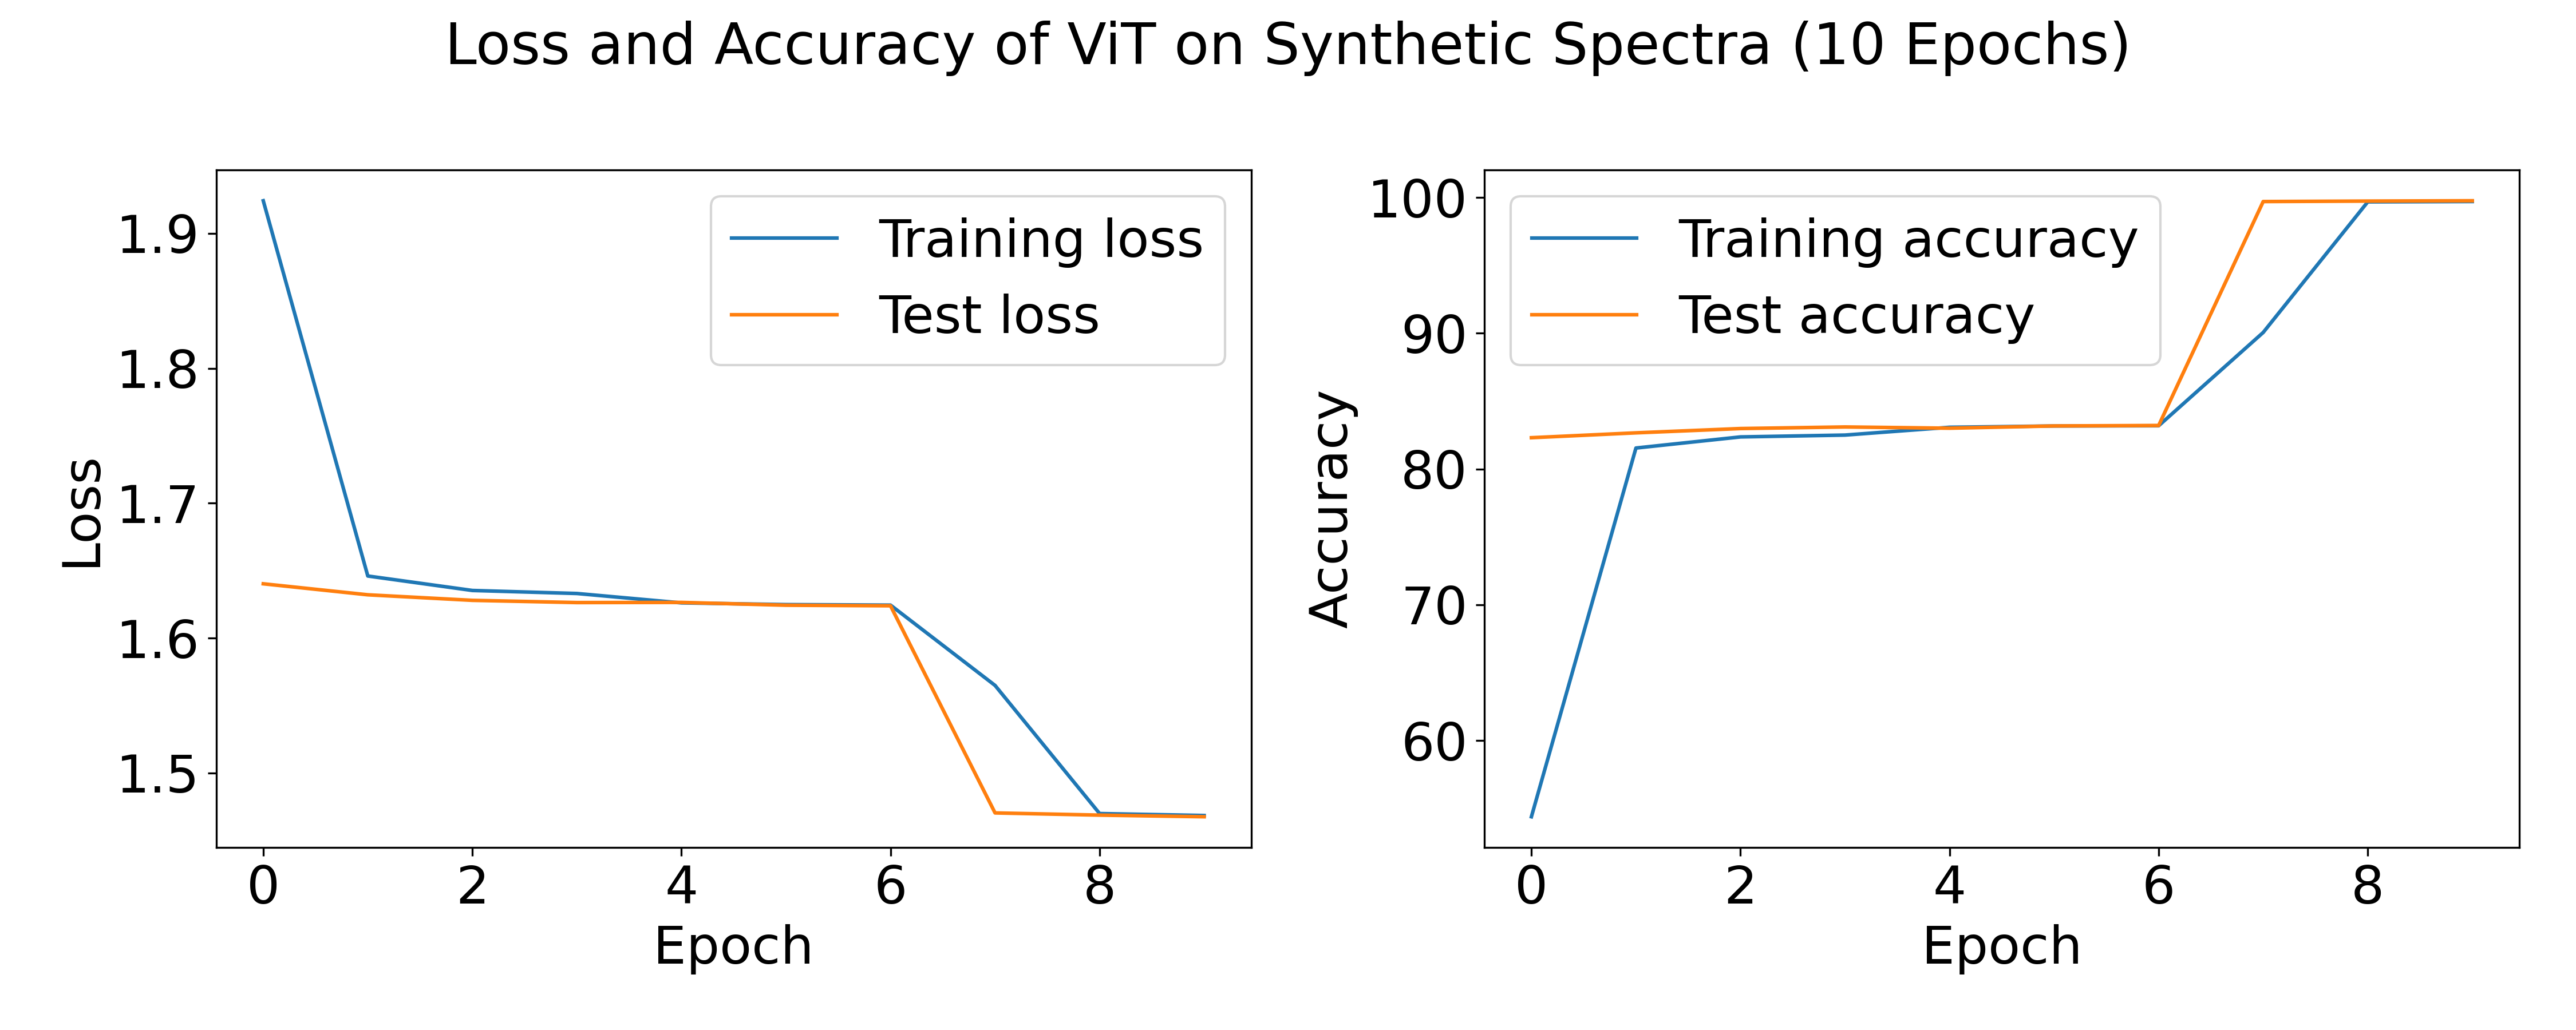
\includegraphics[width=11cm]{figures/pre_testing/SNR10_training_epoch.png}}
    \caption[Verification of ViT: Synthetic Dataset]{Training of Spectral ViT on synthetic datasets. The model was able to reach 100\% accuracy on the test set of SNR=10 (top), 
    but failed to reach an accuracy of 50\% on the test set of SNR=2 (bottom).}
\label{fig:synth_spectra_training}
\end{figure}



\section{Creation of Synthetic DESI Spectra}
\label{sec:synth_data}
Once we demonstrated the Spectral ViT architecture was training effectively on simple synthetic data,
the architecture was trained on DESI data. In order to create a large enough training 
set, observed DESI spectra were used as a base to create synthetic spectra. The process of 
generating the spectra is explained in detail by \textcite{Sepeku2022}, but a brief 
description is provided below. 

\begin{figure}[t!]
    \centering
    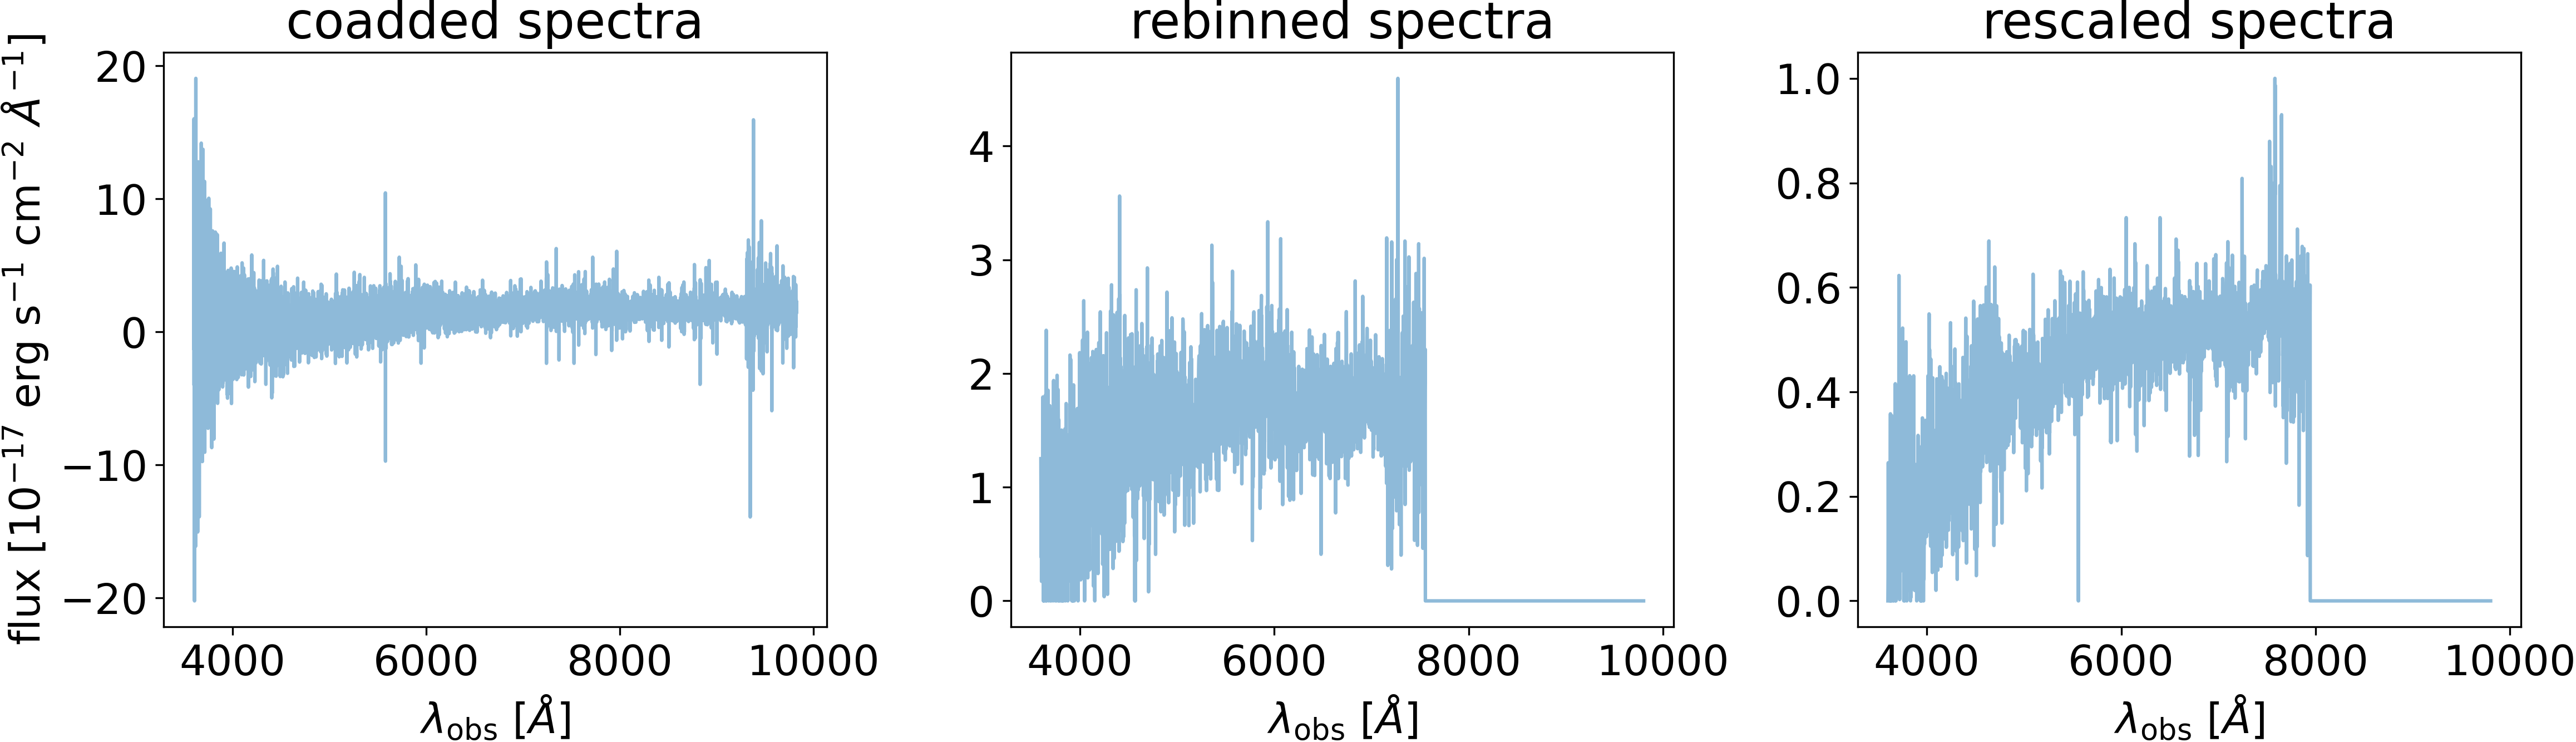
\includegraphics[width=\textwidth]{figures/preprocess/3600_Zcorrected_spectra.png}
    \caption[Spectra Pre-Processing --  Redshift Corrected]{DESI synthetic spectra undergoing pre-processing. The different bands
    are first coadded together (left image). This is then  corrected to the galaxies rest frame and separated into 3600 
    log-scale bins (center image). Finally, the sample is normalized between 0 and 1 (right image)}
    \label{fig:spectra_preproc}
\end{figure} 
Observed DESI BGS spectra were used to construct the training and validation samples. 
Type Ia supernovae were simulated using the \texttt{sncosmo} package \parencite{sncosmo}, and the templates 
provided by \textcite{Hsiao2007}. For core-collapse SNe, the spectra were simulated based 
on models produced by \textcite{Vincenzi2019}. Measured BGS spectra were randomly drawn from DESI observations, and the Ia and core-collapse templates were simulated in {\tt desisim} using the same observing conditions (seeing, transparency, moon illumination, airmass) as the measured spectra. The simulated transient spectra were also allowed to vary in the $r$ band relative to the ``host'' galaxy spectrum to simulate a variety of observing conditions, such as the transient being located off the fiber axis (resulting in a faint signal) or close to the fiber axis (resulting in a relatively strong signal). The simulated transients were then coadded to the corresponding ``host'' spectra and saved to a FITS file in the DESI spectrum format.

\begin{figure}[b!]
    \centering
    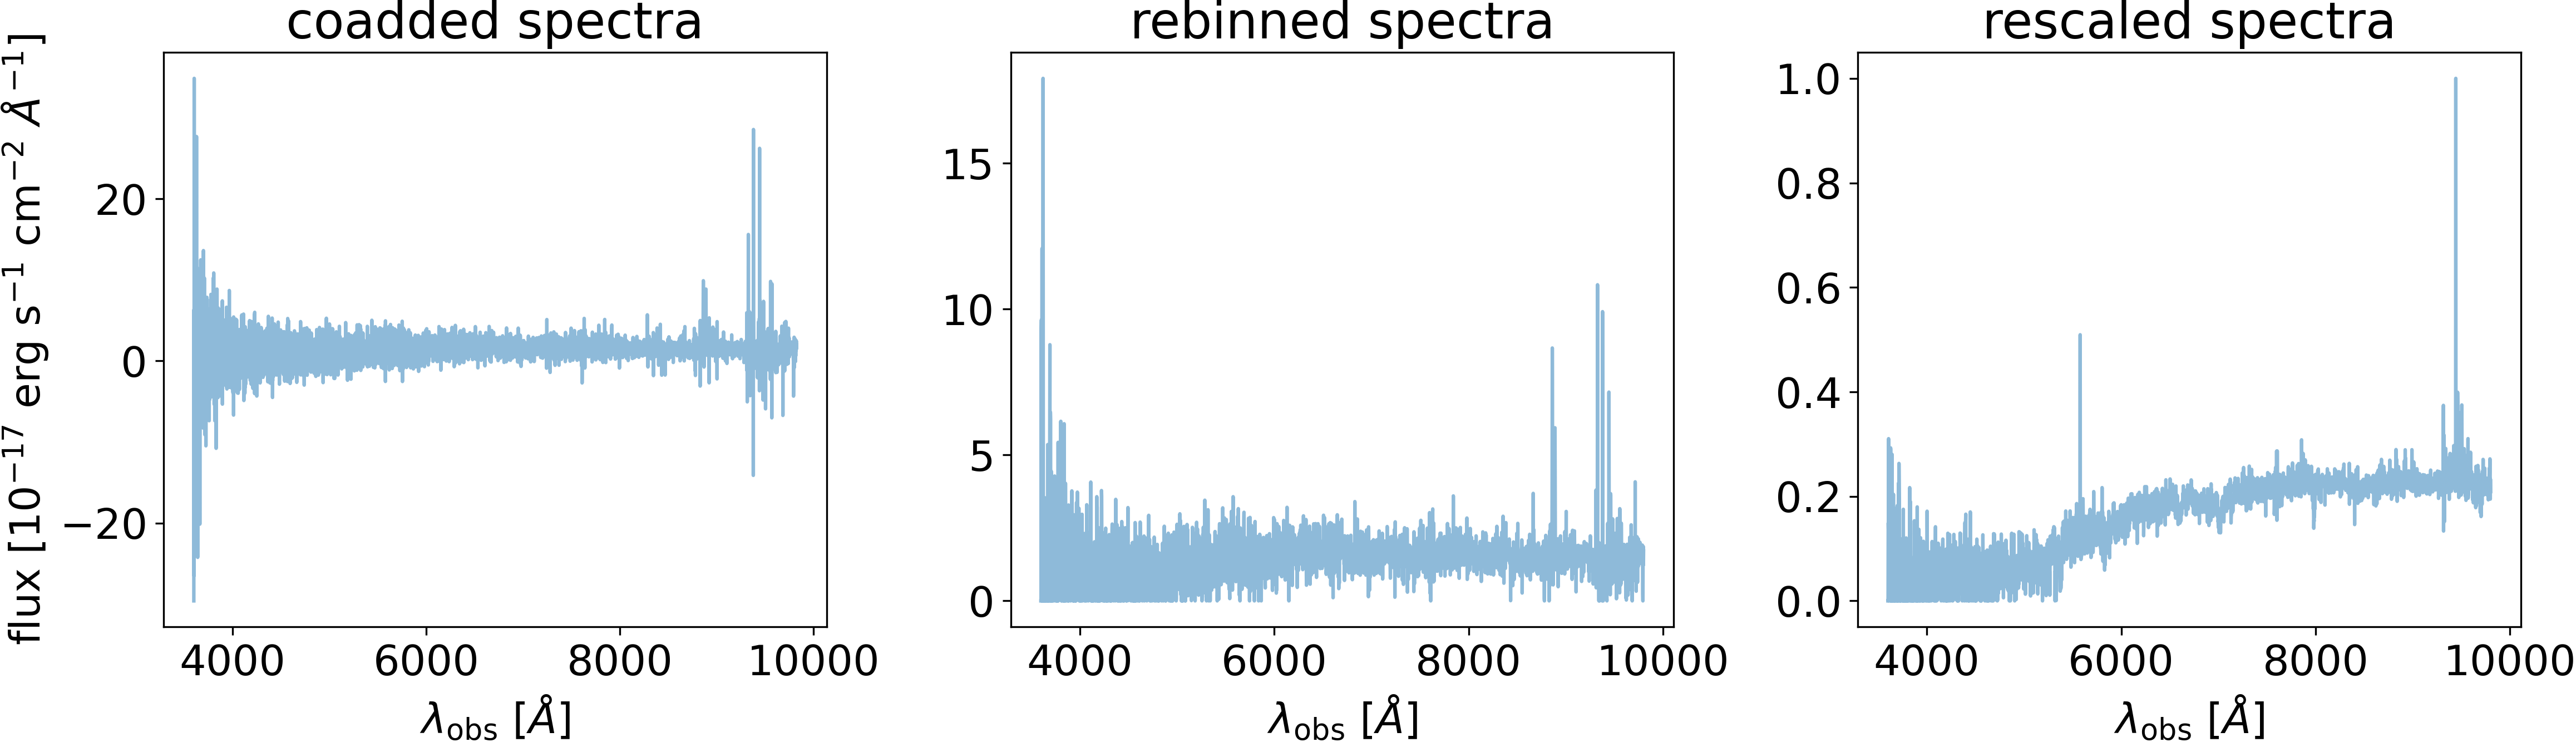
\includegraphics[width=\textwidth]{figures/preprocess/3600_Zrestframe_spectra.png}
    \caption[Spectra Pre-Processing -- Not Redshift Corrected]{DESI synthetic spectra undergoing pre-processing. 
    The different bands are first coadded together (left image). This is then separated 
    into 3600 log-scale bins without any redshift correction (center image). Finally, 
    the sample is normalized between 0 and 1 (right image)}
    \label{fig:sepctra_preproc_nored}
\end{figure} 
\subsection{Pre-Processing of DESI Spectra}
\label{ssec:preprocess}
% All of preprocessing including z correction and downsampling 
Once the spectra were created and saved as DESI files, they needed to be 
extracted, preprocessed, and split into training, testing, and validation sets. Then they could be saved and used to train the Spectral ViT.
The preprocessing method developed by \textcite{wasserman2021, Sepeku2022} was used, and includes four main steps: camera coaddition, redshift correction, rebinning/downsampling, and flux normalization/rescaling. 

The reduced spectra, a table of best-fit redshifts from redrock, and a set of redrock templates and 
coefficients are provided by the DESI pipeline in the form of a FITS file \parencite{Pence2010, Guy2023}.
After the spectra between the different cameras are coadded, the best redshift identified by redrock is used to shift the spectra back into the 
``host'' galaxies' rest frames. 
\begin{table}[t!]
    \small
    \centering
    \sffamily
    \begin{tabular}{lc}
	\toprule
    \textbf{Hyperparameter} & \textbf{Value} \\
    \midrule
    Learning Rate & 0.00004135238172950965 \\ 
    \midrule
    Regularization & 0.06 \\ 
    \midrule
    Dropout Rate & 0.40904759925886294\\
    \midrule
    Batch Size & 50 \\
    \bottomrule
\end{tabular}

    \caption{Hyperparameters of the CNN used to classify DESI spectra. CNN adapted 
    from \textcite{Sepeku2022}.}
    \label{tab:cnn_hyperparameters}
\end{table}
\begin{figure}[b!]
    \centering
    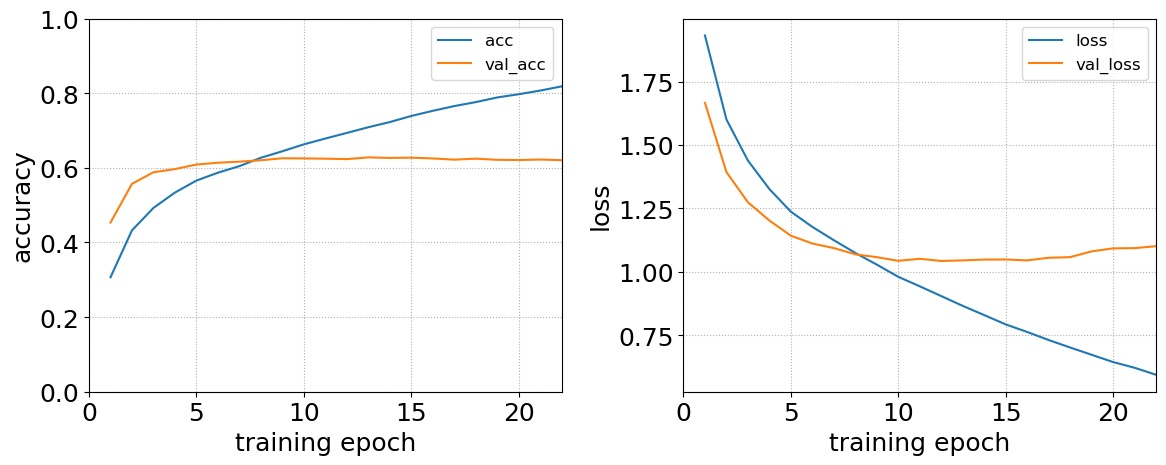
\includegraphics[width=.85\linewidth]{figures/cnn/cnn_training_history.jpg}
    \caption[CNN Training]{Training of the CNN on synthetic DESI spectra.}
    \label{fig:cnn_training}
\end{figure}
Following de-redshifting, all artifacts in the spectra (masks, bad pixels, etc.) are removed. The spectra are then downsampled to a user-defined resolution (default is 3600 bins) and normalized to rescale the minimum and maximum flux values to 0 and 1. 
Each of these steps is shown in succession in Figure~\ref{fig:spectra_preproc} for a 
redshift-corrected spectrum with 3600 bins, and in Figure~\ref{fig:sepctra_preproc_nored} for a non-redshift corrected spectrum, also with 3600 bins. 

\subsection{Transformer Training}
\label{sec:transformer_training}
\begin{table}[t!]
    \small
    \centering
    \sffamily
    \begin{tabular}{lcc}
	\toprule
    \textbf{Hyperparameter} & \textbf{Smaller Architecture} & \textbf{Larger Architecture} \\
    \midrule
    Learning Rate & 0.0001 & 0.01 \\ 
    \midrule
    Batch Size & 16 & 16 \\
    \midrule
    Blocks & 4 & 4 \\
    Heads & 5 & 12 \\
    Hidden Dimension & 25 & 72 \\
    \bottomrule
\end{tabular}

    \caption{Hyperparameters of the smaller and larger Spectral ViT architecture used to classify DESI spectra.}
    \label{tab:t_hyper}
\end{table}

\begin{figure}[b!]
    \centering
    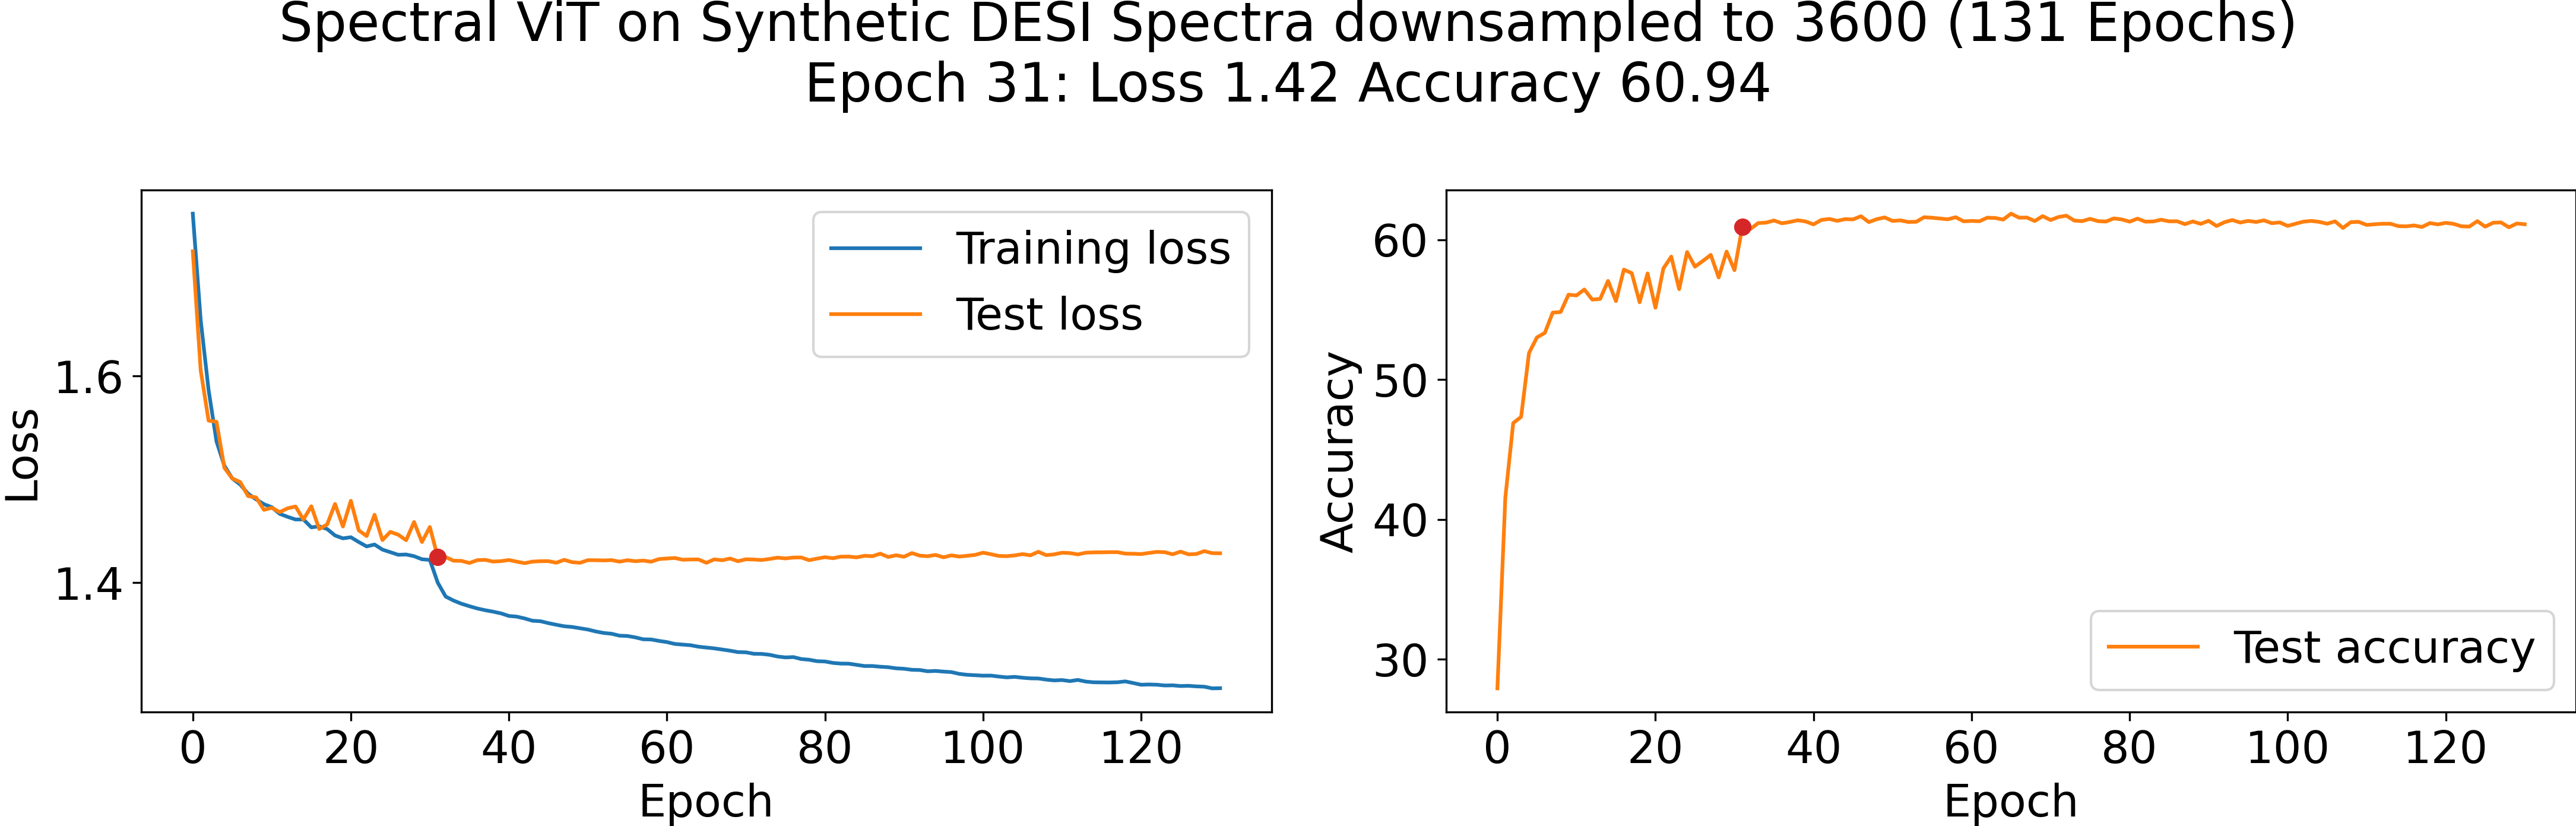
\includegraphics[width=.85\linewidth]{figures/v1_real/vit_model_V1_original_redotraining_new.png}
    \caption[Training of Spectral ViT: V1]{Training of the small architecture on redshift-corrected spectra downsampled to 3600 bins. Over-fitting was determined to have occurred by Epoch 31.}
    \label{fig:vit1_training}
\end{figure}
For the CNN datasets, the spectra were split into 2D arrays of equal height and width 
(i.e. for spectra of length 3600, the arrays would have a shape of $60\times60$). 
After this, the spectra were divided into training, testing, and validation samples comprising 60\%, 20\%, and 20\% of the total dataset.


\begin{figure}[t!]
    \centering
    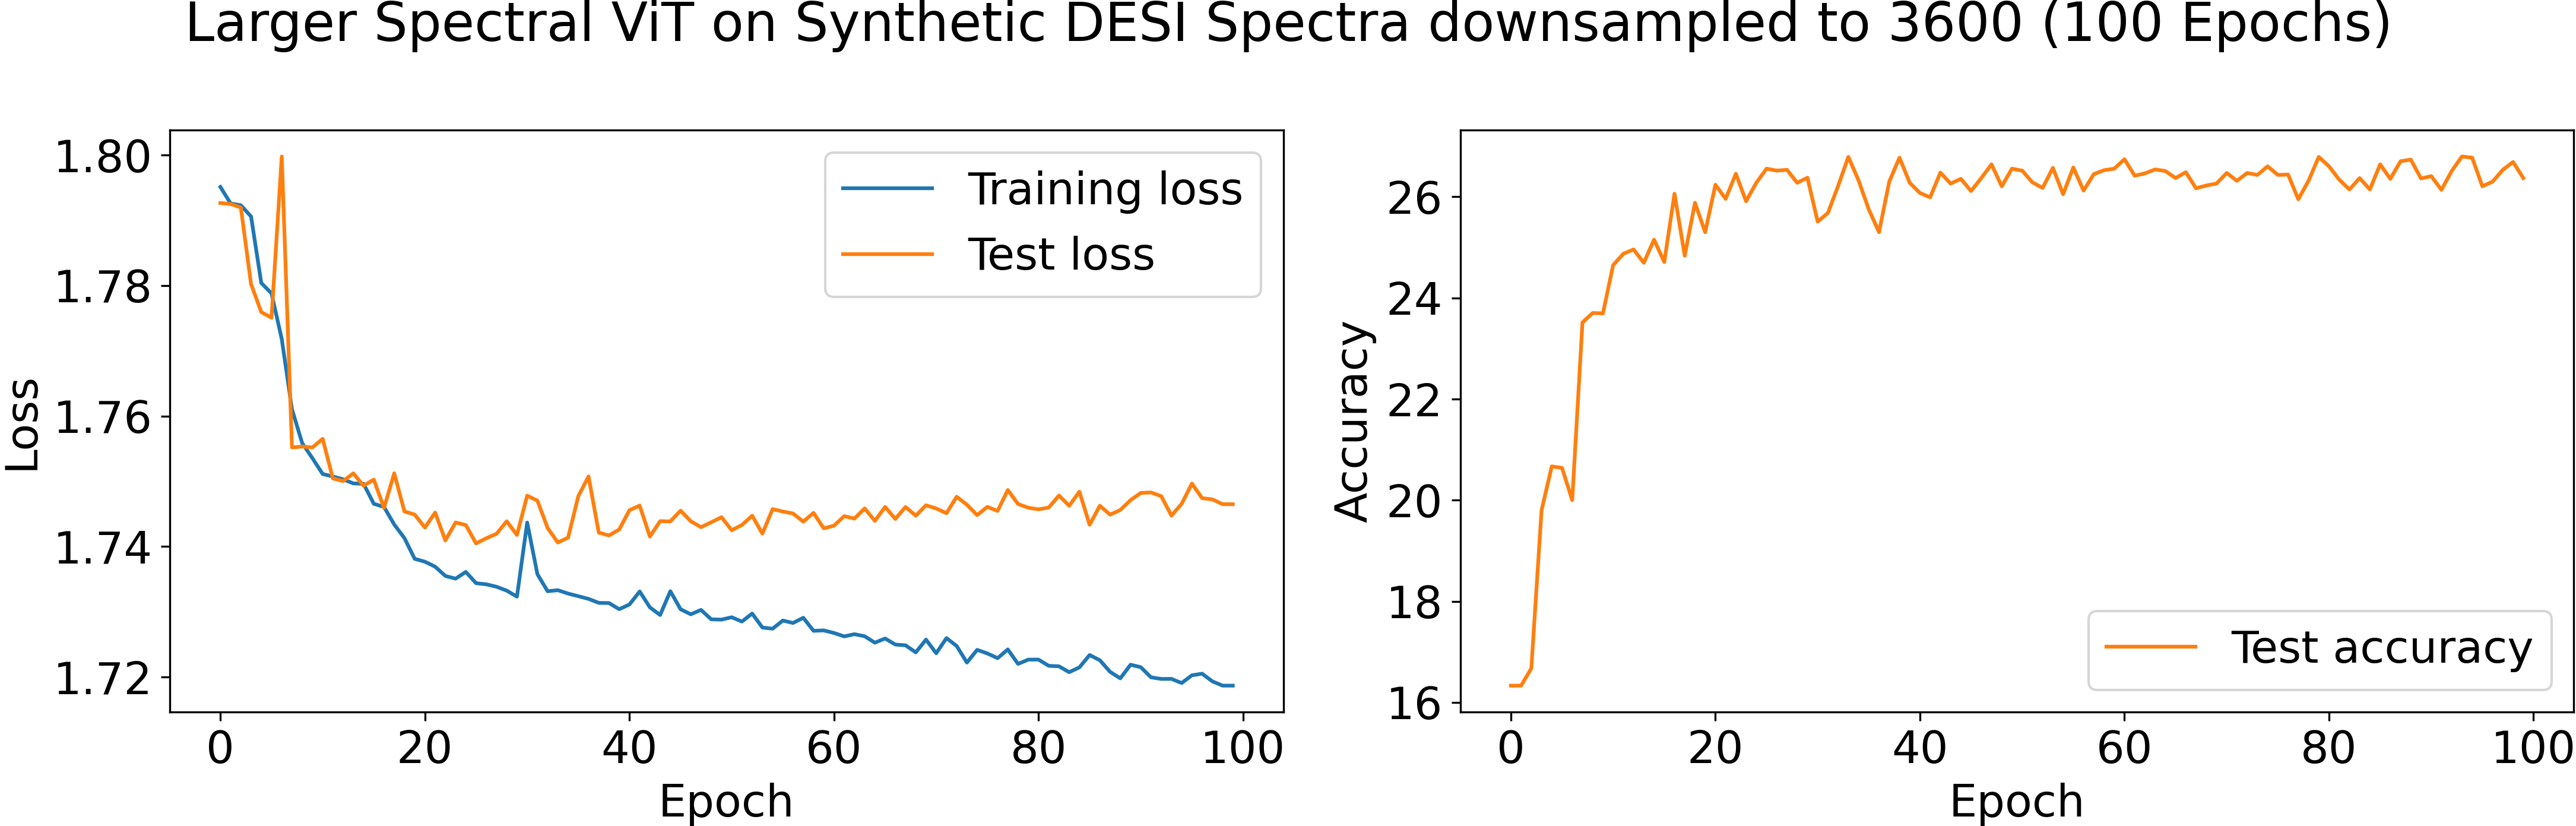
\includegraphics[width=.85\linewidth]{figures/v1_real/vit_model_V1_bigtraining_new.png}
    \caption[Training of Spectral ViT: V1 Big]{Training of the large architecture on Redshift-corrected spectra downsampled to 3600 bins. No convergence above random guessing was observed. }
    \label{fig:vit1_big_training}
\end{figure}
Two Spectral ViT architectures were trained on the same synthetic DESI spectra as the CNN.
The first Spectral ViT architecture was smaller than the second. The properties 
of both are shown in Table~\ref{tab:t_hyper}. 

\section{Training of Neural Networks}
\label{sec:training} 
\subsection{CNN Training}
\label{ssec:cnn_training}
The CNN architecture was developed by \textcite{Sepeku2022}, and has properties 
\begin{figure}[hb!]
    \centering
    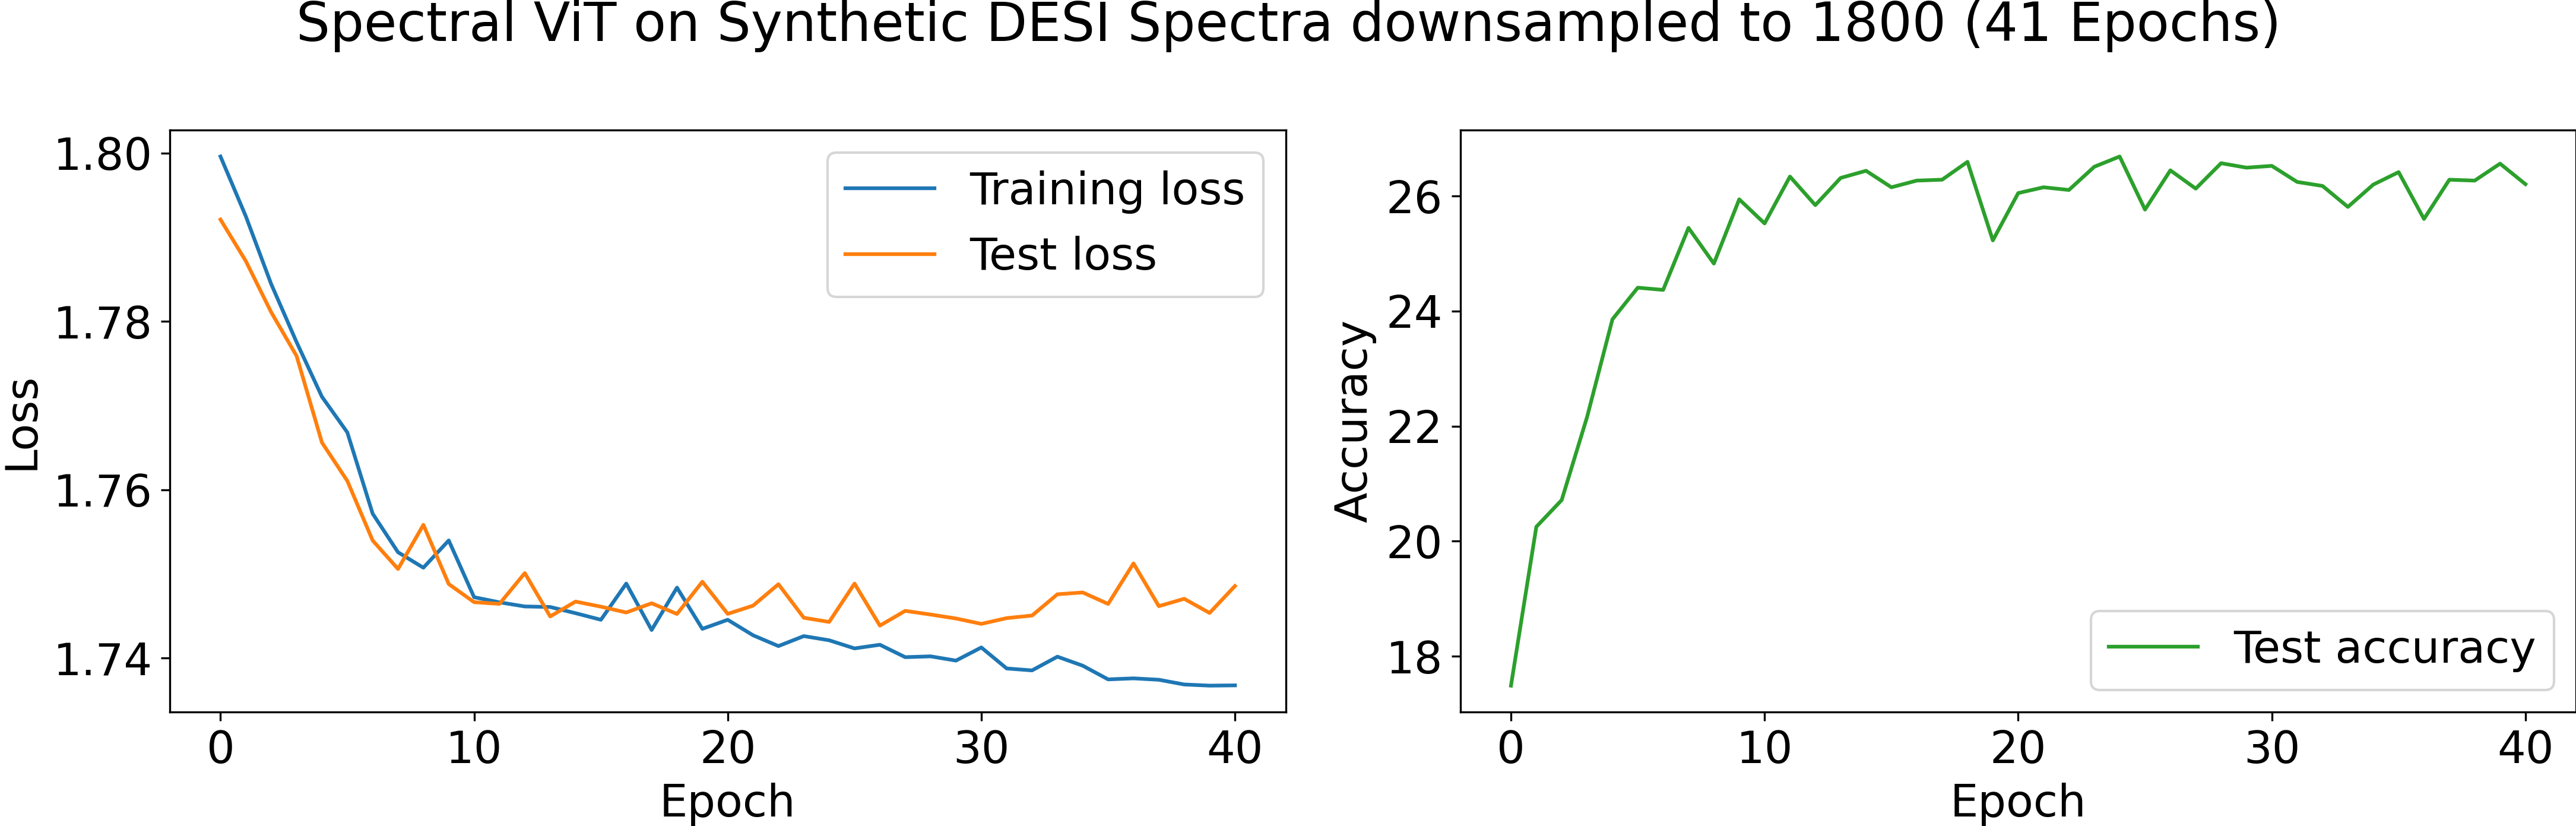
\includegraphics[width=.85\linewidth]{figures/vit_model_V1.2training_new.png}
    \caption[Training of Spectral ViT: V1.2]{Training of the small architecture on Redshift-corrected spectra downsampled to 1800 bins. No convergence above random guessing was observed. }
    \label{fig:vit1.2_training}
\end{figure}
shown in Table~\ref{fig:cnn_architecture}.
This CNN was trained for a maximum of 50 epochs, with a batch size of 50, and 
non-variable hyperparameters (Table~\ref{tab:cnn_hyperparameters}). 
The timeline of the training of the CNN architecture is shown in Fig.~\ref{fig:cnn_training}.



Both architectures were initially trained on spectra downsampled to 3600 bins. As shown in Figure~\ref{fig:vit1_training}, 
the smaller architecture was able to train effectively, reaching a test accuracy of 60.94\% after approximately 31 
epochs. The larger architecture did not converge as well, only reaching a test accuracy of around 26\% before 
overfitting, as shown in Figure~\ref{fig:vit1_big_training}. Therefore, the smaller architecture was chosen for further testing.

\begin{figure}[t!]
    \centering
    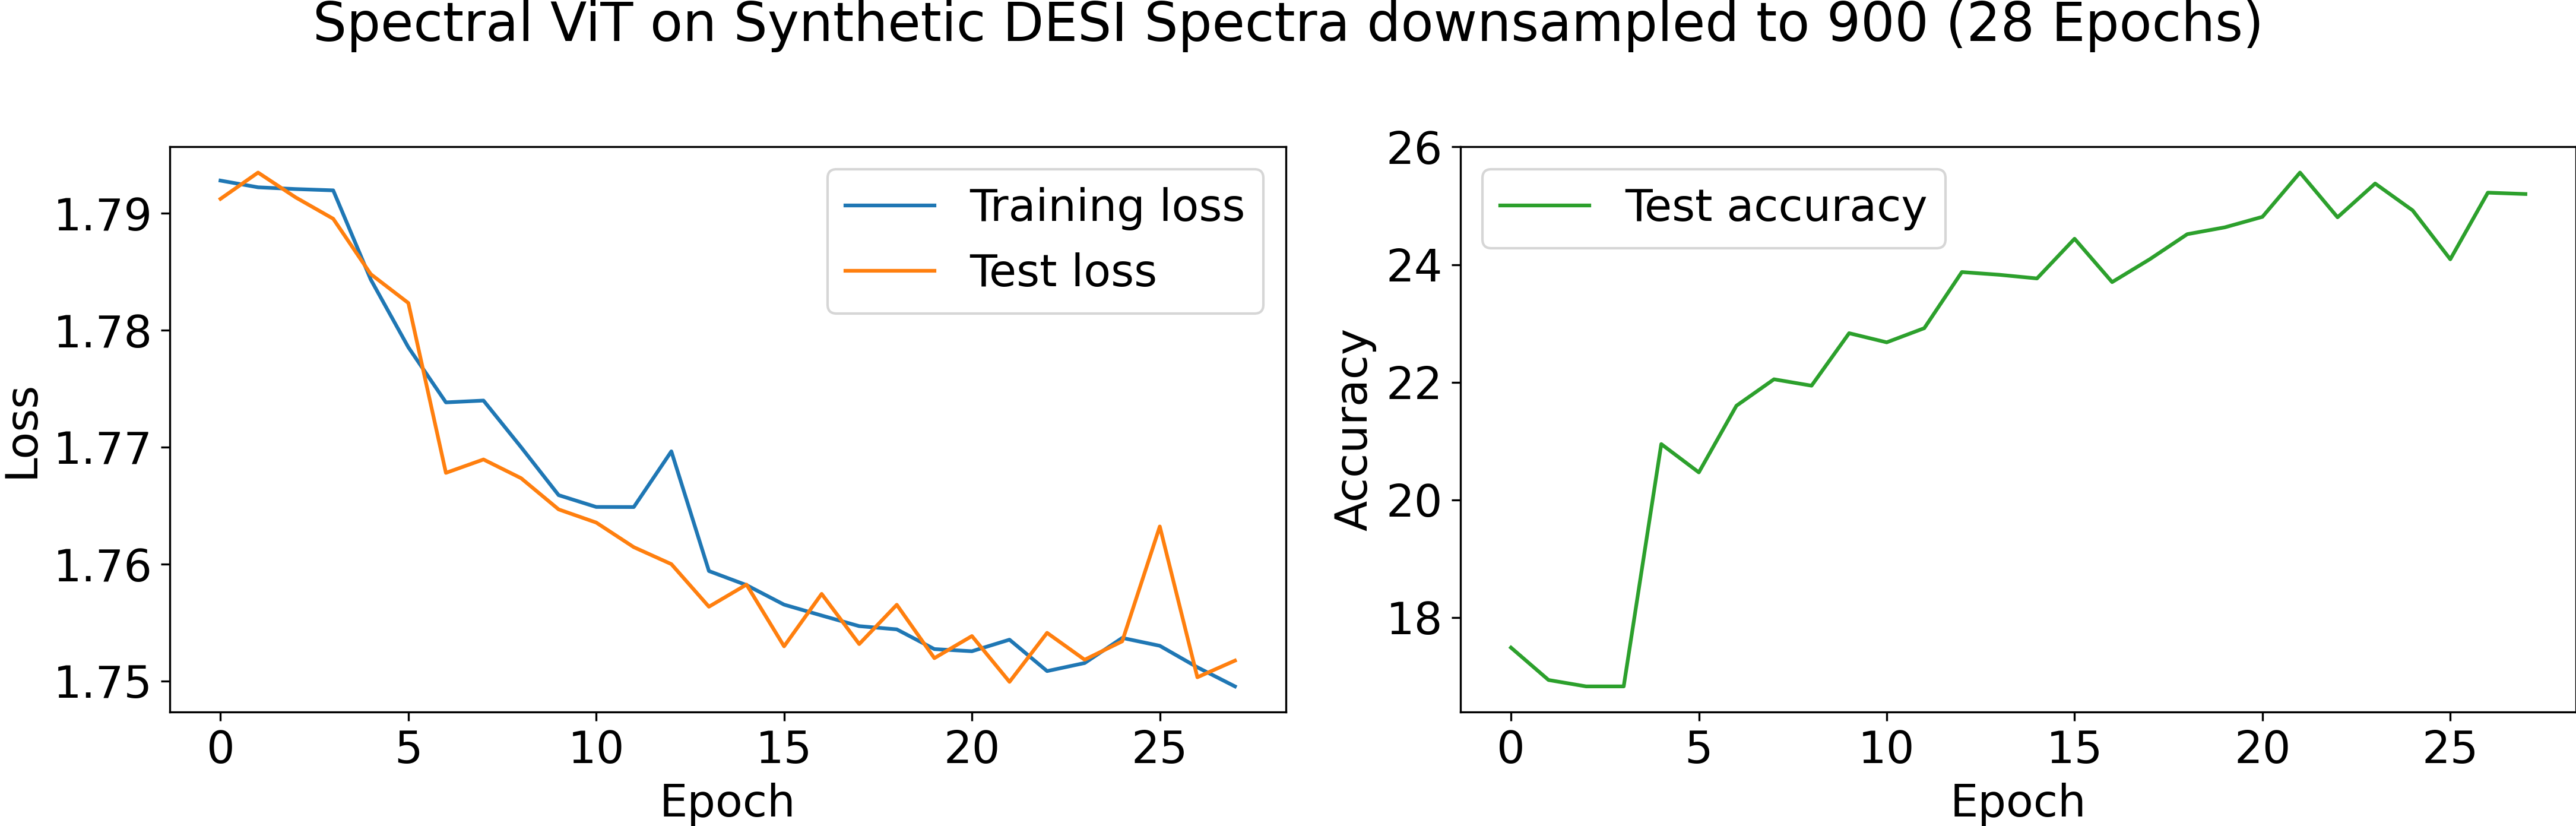
\includegraphics[width=.85\linewidth]{figures/vit_model_V1.3_muchsmallermodeltraining_new.png}
    \caption[Training of Spectral ViT: V1.3]{Training of the small architecture on Redshift-corrected spectra downsampled to 900 bins. No convergence above random guessing was observed. }
    \label{fig:vit1.3_training}
\end{figure}



To explore the effect of the dimensionality of the input data on the performance of the Spectral ViT, the smaller architecture was trained on spectra downsampled to 1800 and 900 bins. As shown in Figure~\ref{fig:vit1.2_training} and Figure~\ref{fig:vit1.3_training},
neither variation was able to train as effectively as the original binning. 

\begin{figure}[t!]
    \centering
    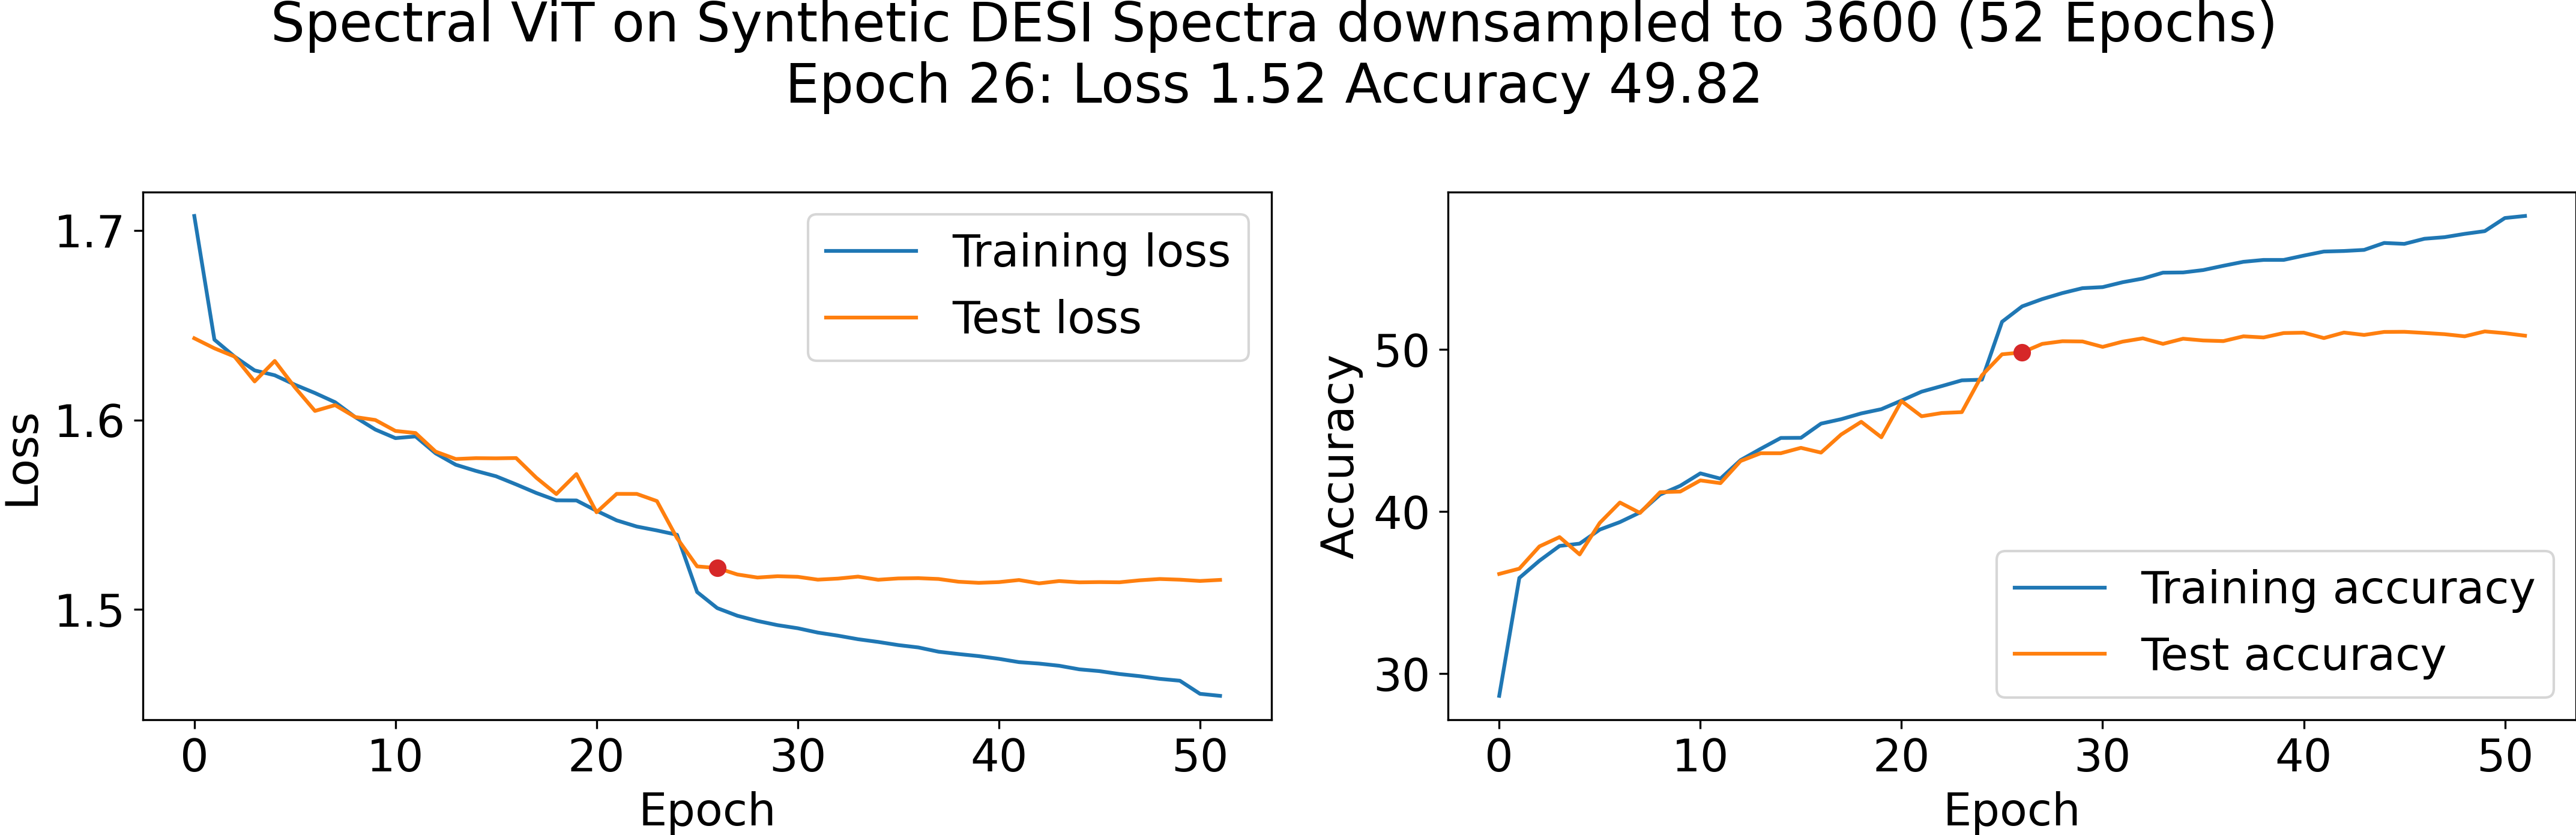
\includegraphics[width=.85\linewidth]{figures/v2_real/vit_model_V2training_new.png}
    \caption[Training of Spectral ViT: V2]{Training of the small architecture on non Redshift-corrected data downsampled to 3600 bins. Over fitting was determined to have occurred by Epoch 26.}
    \label{fig:vit2_training}
\end{figure}
The smaller architecture, using input spectra with 3600 bins, was then trained on the
non-redshift-corrected spectra. As shown in Figure~\ref{fig:vit2_training},
the model was able to train effectively, reaching a test accuracy of 49.82\%. 
This lack of dependence on DESI redshift fitting is promising, as it means that 
the model could be used to classify spectra without the need for the redshift fit. 


